% Workflow overview for Section III (Review Methodology) of tqe.tex.
% Compile with:  pdflatex review_workflow.tex   (run from TQE_Template/figures)
\documentclass[border=1pt]{standalone}
\usepackage{times}
\usepackage{tikz}
\usetikzlibrary{arrows.meta,positioning}
\begin{document}
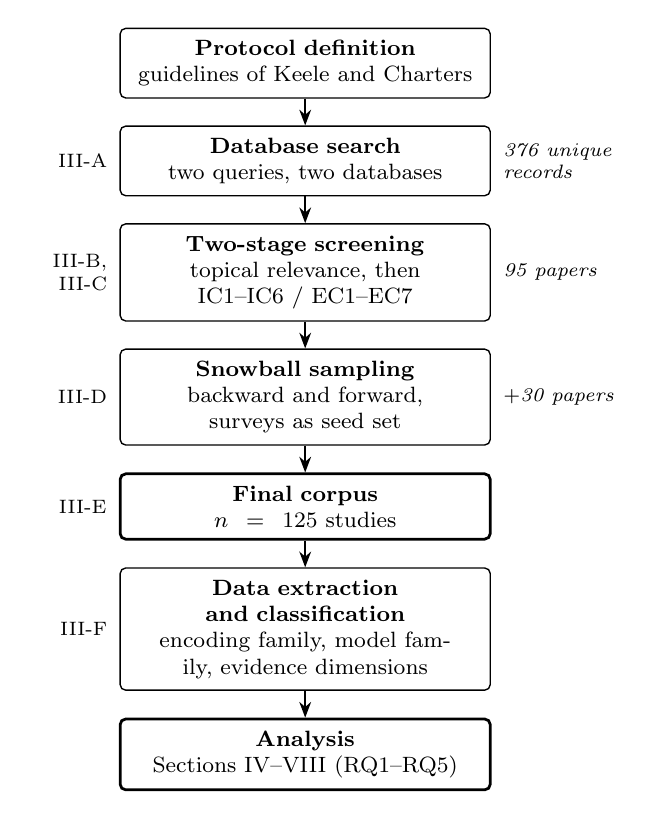
\begin{tikzpicture}[
  font=\footnotesize,
  node distance=3.4mm,
  stage/.style={draw, rounded corners=2pt, align=center, inner sep=1.5mm,
                text width=44mm, line width=0.5pt},
  keystage/.style={stage, line width=1pt},
  flow/.style={-{Stealth[length=2mm]}, line width=0.6pt},
  note/.style={align=left, text width=15mm, font=\scriptsize\itshape, inner sep=0pt},
  tag/.style={align=right, text width=10mm, font=\scriptsize, inner sep=0pt}
]
\node[stage] (proto) {\textbf{Protocol definition} \\ guidelines of Keele and Charters};
\node[stage, below=of proto] (search) {\textbf{Database search} \\ two queries, two databases};
\node[stage, below=of search] (screen) {\textbf{Two-stage screening} \\ topical relevance, then IC1--IC6 / EC1--EC7};
\node[stage, below=of screen] (snow) {\textbf{Snowball sampling} \\ backward and forward, surveys as seed set};
\node[keystage, below=of snow] (corpus) {\textbf{Final corpus} \\ $n = 125$ studies};
\node[stage, below=of corpus] (extract) {\textbf{Data extraction and classification} \\ encoding family, model family, evidence dimensions};
\node[keystage, below=of extract] (analysis) {\textbf{Analysis} \\ Sections IV--VIII (RQ1--RQ5)};

\foreach \a/\b in {proto/search, search/screen, screen/snow, snow/corpus, corpus/extract, extract/analysis}
  \draw[flow] (\a) -- (\b);

\node[note, right=1.5mm of search] {376 unique records};
\node[note, right=1.5mm of screen] {95 papers};
\node[note, right=1.5mm of snow] {$+$30 papers};

\node[tag, left=1.5mm of search] {III-A};
\node[tag, left=1.5mm of screen] {III-B, III-C};
\node[tag, left=1.5mm of snow] {III-D};
\node[tag, left=1.5mm of corpus] {III-E};
\node[tag, left=1.5mm of extract] {III-F};
\end{tikzpicture}
\end{document}
